\maketitle
\tableofcontents
\newpage
\section{Introduction}
  \indent Nowadays, antennas have been using in every wireless communication systems. It have been found out that microstrip patch is one of the most popular\cite{AkS} in the world. Also, the patch antenna is cost-effective and easy to fabricate\cite{AtT}. Many design approaches have been revealed for antenna engineers to follow the procedure. In order to obtain the precise dimension, a deep analysis might've be engaged.
  \indent A phased array is the set of antennas that could be a formation as a line or a planar which could steer its beam electrically\cite{CoB:05} which means that the direction of the antenna can be control wthout moving any of the mechanic part. Therefore, this proposal is aiming on two of very interesting technologies in this era.

\section{Objectives}
  \indent The propose of this work is mainly focus on analyzing and designing the 5.6 GHz planar phased array antenna based on methods which have been analyzed, formulated or derived in the past. 

\section{Methodology}
  \indent This section will provide a full analysis of designing a microstrip antenna and a phased array antenna.

  \subsection{Dimension Design of the Microstrip Antenna}
    \indent a dimension of microstrip antenna can be designed easily with this expressions\cite{NoK:05}.
    \begin{equation}
      L = \frac{c}{2f_0\sqrt{\epsilon_r\mu_r}} - 2\Delta l 
      W = \frac{c}{2f_0}
    \end{equation}
    \indent where $L$ and $W$ are the dimensions of an antenna\\[1ex]
    \indent $f_0$ is the resonance frequency\\[1ex]
    \indent $\epsilon_r$ is the relative dielectric constant\\[1ex]
    \indent $\mu_r$ is the relative magnetic constant\\[1ex]
    \indent $c$ is the speed of light in free space\\[1ex]
    \indent $\Delta l$ is the fringing effect at the edge of the antenna
    \indent However from \cite{CoB:05} the best width should be
    \begin{equation}
      W = \frac {1} {2 f_r \sqrt{\mu_{0} \epsilon_{0}}}\sqrt{\frac{2}{\epsilon_{r} + 1}} = \frac{\upsilon_{0}}{2f_{r}}\sqrt{\frac{2}{\epsilon_{r} + 1}}
    \end{equation}
    \indent where $\upsilon_{0}$ is the free-space velocity of light

  \subsection{Fringing Effect of the Microstrip Antenna}
    \subsubsection {Length Extension} 
    \begin{equation}
      \frac{\Delta l}{h}=0.412\frac{(\epsilon_{r(eff)}+0.3)(\frac{W}{h} + 0.264)}{(\epsilon_{r(eff)}-0.258)(\frac{W}{h} + 0.8)}
    \end{equation}
    \indent The length is extended by $\Delta L$ on both side so $L_{eff} = L + 2\Delta L$\\

  \subsection{Resonance frequency}
    \indent In $TM_{010}$ mode, the resonant frequency is given by
    \begin{equation}  
      f_{r(010)} =  \frac{1}{2 L\sqrt{\epsilon_{r}}\sqrt{\epsilon_{\mu_{0}\epsilon_{0}}}}= \frac{\upsilon_{0}}{2L\sqrt{\epsilon_{r}}}
    \end{equation}
    \indent With fringing effect, the equation will be given by
    \begin{equation} 
      f_{r(010)} =  \frac{1}{2 L_{eff}\sqrt{\epsilon_{r(eff))}}\sqrt{\epsilon_{\mu_{0}\epsilon_{0}}}}=\frac{1}{2(L + 2\Delta L)\sqrt{\epsilon_{r(eff)}}\sqrt{\epsilon_{\mu_{0}\epsilon_{0}}}}
    \end{equation}

  \subsection{Q Factor}
  \indent Quality factor desctibes the quotient between the power stored in the reactive field and the radiated power
  \subsection{Radiation Resistance}
    \indent Radiation Resistance defines how 

  \subsection{Bandwidth}

  \subsection{Radiation Pattern}

  \subsection{Transmission Line Model}

  \subsection{Cavity Line Model}

  \subsection{Phased Array Antenna}
    In phased array antenna principle, there are 2 main factor in the equations. First one is an element factor which is the factor that come from only one antenna itself and the another factor is called array factor which is come from the effect of multiple antennas combining together.
    \begin{equation} 
      S(\vartheta)=S_{e}(\vartheta)S_a(\vartheta)  \label{ii}
    \end{equation}
      Whereas \\[1ex]
      \indent $S_{e}$ is a radiation pattern from only one element\\
      \indent $S_{a}$ is a element factor with
      \begin{equation} 
        S_{a}(\vartheta) = \sum\limits_{i=1}^K a_{i}e^{jk(K-i)dsin(\vartheta)}
      \end{equation}
      \indent $a_{i}$ is an amplitude taper.\\
      \indent $K$ is a number of array antenna.\\
      \indent $d$ is a distance of each antenna.\\
      \indent $\vartheta$ is a wavefront angle

\pagebreak

\section{Preliminary results}
  \subsection{Microstrip Antenna}
    \begin{figure}[h]
      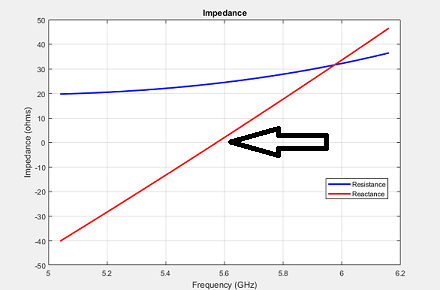
\includegraphics{Impedance.png}
      \centering
      \caption{The designed antenna's impedance should have approximately 0 Ohm reactance at 5.6 GHz}
      \label{fig:1}
    \end{figure}

    \begin{figure}[h]
      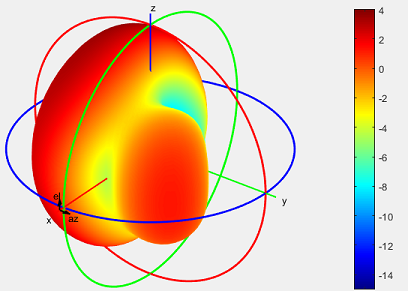
\includegraphics{Radiation_pattern}
      \centering
      \caption{The designed antenna's radiation pattern should have clear directivity}
      \label{fig:2}
    \end{figure}

\pagebreak

  \subsection{Array Antenna Patern}
    \begin{figure}[h]
      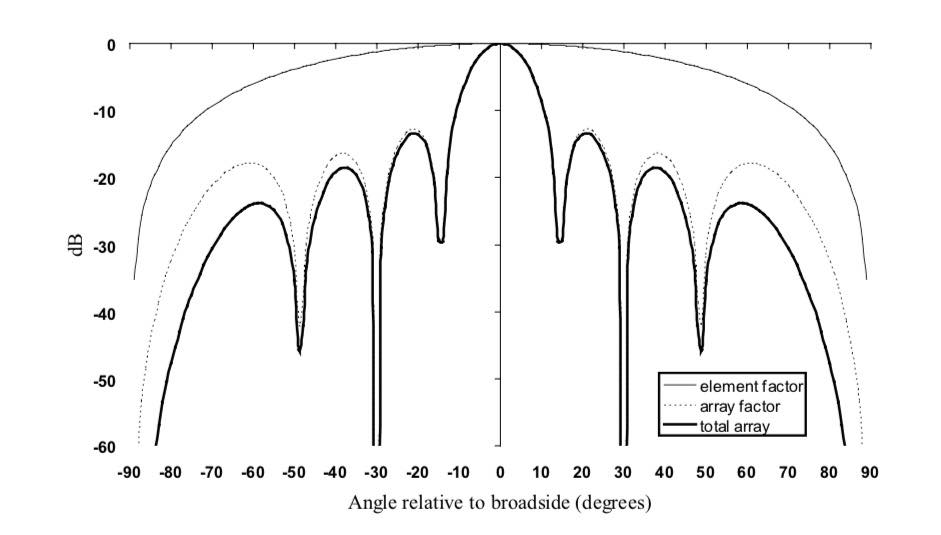
\includegraphics[scale=0.5]{no_taper}
      \centering
      \caption{Power radiation pattern without amplitude taper aka. $\forall a_{i} = 1$}
      \label{fig:3}
    \end{figure}

    \begin{figure}[h]
      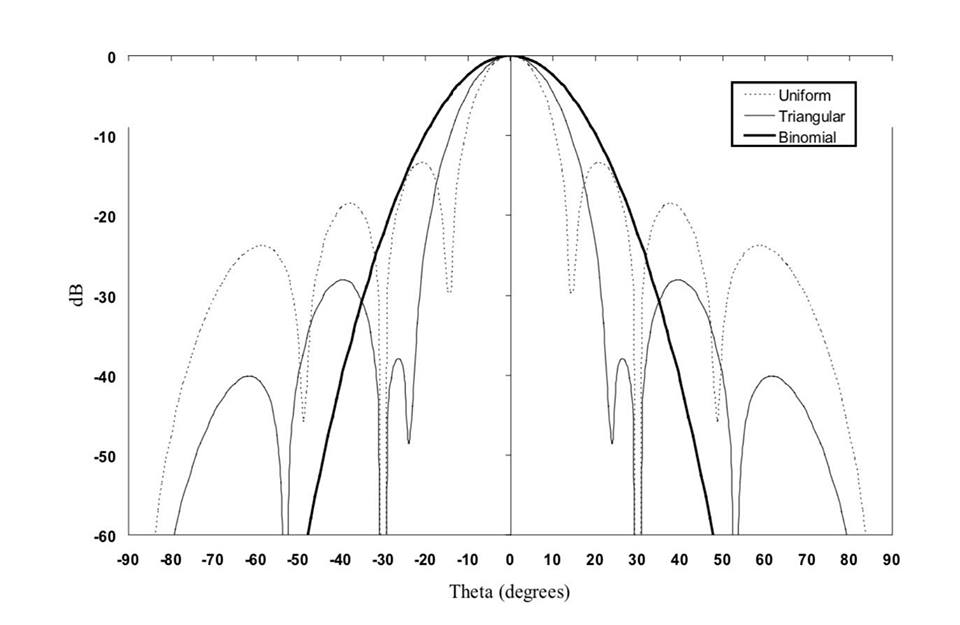
\includegraphics[ scale=0.5]{with_taper}
      \centering
      \caption{Power radiation pattern with amplitude taper of each type}
      \label{fig:4}
    \end{figure}

\pagebreak

\section{Project overview}
  \subsection{Scope of work}
    \begin{itemize}
      \item Analyze the microstrip antenna and phased array antenna
      \item Design the microstrip antenna and phased array antenna
      \item Simulate the microstrip antenna and phased array antenna
      \item Create the microstrip antenna and phased array antenna
      \item Test the microstrip antenna and phased array antenna
    \end{itemize}

  \subsection{Expected outcomes}
    \indent A physical and a simulation file of a phased array antenna with electronic controlled devices and its experimental document

  \newpage

  \bibliography{ref} 
  \bibliographystyle{ieeetr}